\chapter{Graph Data Structures}

\section{Introduction}
A \textbf{graph} is a data structure used to represent a set of objects (called \textbf{vertices} or \textbf{nodes}) and the relationships between them (called \textbf{edges}). Graphs are widely used to model many real-world problems such as social networks, transportation systems, and web page link structures. Depending on the application, graphs can be:
\begin{itemize}
    \item \textbf{Directed} (where edges have a direction).
    \item \textbf{Undirected} (where edges are bidirectional).
    \item \textbf{Weighted} (if edges carry a cost, distance, or other metric).
\end{itemize}

\section{Definition, Terminology, and Formulas}
A graph \( G \) is defined as a pair \( (V, E) \), where:
\begin{itemize}
    \item \( V \) is a non-empty set of vertices.
    \item \( E \) is a set of edges, where each edge is a pair (or ordered pair in directed graphs) of vertices.
\end{itemize}

\subsection{Key Terminology}
\begin{description}
    \item[Vertex (Node):] An individual object in the graph.
    \item[Edge: ] A connection between two vertices.
    \item[Adjacent: ] Two vertices that are directly connected by an edge.
    \item[Degree: ] For an undirected graph, the degree of a vertex is the number of edges incident on it. In directed graphs, we differentiate between \textbf{in-degree} and \textbf{out-degree}.
    \item[Path: ] A sequence of vertices connected by edges.
    \item[Cycle: ] A path that starts and ends at the same vertex without repeating an edge.
    \item[Connectivity: ] A graph is connected if there is a path between any two vertices.
\end{description}

\subsection{Useful Formulas}
\begin{itemize}
    \item \textbf{Handshaking Lemma (Undirected):} 
    \[
    \sum_{v \in V} \text{degree}(v) = 2|E|
    \]
    \item \textbf{Directed Graph Degree Relationship:}
    \[
    \sum_{v \in V} \text{in-degree}(v) = \sum_{v \in V} \text{out-degree}(v) = |E|
    \]
    \item \textbf{Path Length:} The length of a path is defined as the number of edges in the path.
\end{itemize}

\section{Graph Representations}
Graphs can be represented in several ways. The two primary methods are:

\subsection{Adjacency Matrix}
An adjacency matrix is a 2D array \( A \) of size \( |V| \times |V| \) where:
\[
A[i][j] = \begin{cases}
1 & \text{if there is an edge from vertex } i \text{ to vertex } j, \\
0 & \text{otherwise.}
\end{cases}
\]
For weighted graphs, the entry may store the edge weight instead of 1 (with a special value such as \(\infty\) or 0 indicating no edge).

\subsection{Adjacency List}
An adjacency list represents the graph as an array (or vector) of lists. The list at index \( i \) contains all vertices adjacent to vertex \( i \). This representation is especially space-efficient for sparse graphs.

\subsection{Edge List}
An edge list is simply a list of all edges. Each edge is represented by a pair (or triple for weighted graphs) of vertices:
\[
\text{Edge List } = \{(u,v) \mid u, v \in V\}
\]
This representation is simple and is often used as an intermediate step in algorithms like Kruskal's for finding minimum spanning trees.

\section{Types of Graphs and Detailed Diagrams}
Graphs can be categorized based on the nature of their edges and vertices:

\subsection{Undirected Graph}
In an undirected graph, the edges do not have a direction. An edge between vertices \( u \) and \( v \) is represented as \( \{u, v\} \).

\textbf{Diagram:}
\begin{center}
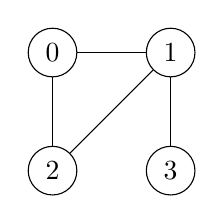
\begin{tikzpicture}[node distance=1.5cm, auto]
    \node[draw, circle] (v0) {0};
    \node[draw, circle, right of=v0] (v1) {1};
    \node[draw, circle, below of=v0] (v2) {2};
    \node[draw, circle, right of=v2] (v3) {3};
    \draw (v0) -- (v1);
    \draw (v0) -- (v2);
    \draw (v1) -- (v2);
    \draw (v1) -- (v3);
\end{tikzpicture}
\end{center}

\subsection{Directed Graph (Digraph)}
In a directed graph, each edge has a direction. An edge from vertex \( u \) to vertex \( v \) is represented as \( (u, v) \).

\textbf{Diagram:}
\begin{center}
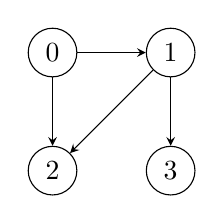
\begin{tikzpicture}[node distance=1.5cm, auto, ->,>=stealth]
    \node[draw, circle] (v0) {0};
    \node[draw, circle, right of=v0] (v1) {1};
    \node[draw, circle, below of=v0] (v2) {2};
    \node[draw, circle, right of=v2] (v3) {3};
    \draw (v0) edge (v1);
    \draw (v0) edge (v2);
    \draw (v1) edge (v2);
    \draw (v1) edge (v3);
\end{tikzpicture}
\end{center}

\subsection{Weighted Graph}
A weighted graph has weights (or costs) associated with each edge. These weights can represent distances, costs, or other metrics.

\textbf{Diagram (Undirected Weighted Graph):}
\begin{center}
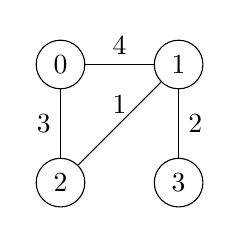
\begin{tikzpicture}[node distance=1.5cm, auto]
    \node[draw, circle] (v0) {0};
    \node[draw, circle, right of=v0] (v1) {1};
    \node[draw, circle, below of=v0] (v2) {2};
    \node[draw, circle, right of=v2] (v3) {3};
    \draw (v0) -- node[midway, above] {4} (v1);
    \draw (v0) -- node[midway, left] {3} (v2);
    \draw (v1) -- node[midway, right] {2} (v3);
    \draw (v1) -- node[midway, above] {1} (v2);
\end{tikzpicture}
\end{center}

\section{C++ Implementations of Graph Representations}
Below are sample C++ implementations for the different graph representations.

\subsection{Adjacency Matrix Implementation}
\begin{lstlisting}[caption={C++ implementation using an Adjacency Matrix}]
#include <iostream>
#include <vector>
using namespace std;

class GraphMatrix {
private:
    int V; // number of vertices
    vector<vector<int>> adjMatrix;
public:
    GraphMatrix(int V) : V(V) {
        adjMatrix.resize(V, vector<int>(V, 0));
    }
    void addEdge(int u, int v, bool undirected = true, int weight = 1) {
        adjMatrix[u][v] = weight;
        if(undirected)
            adjMatrix[v][u] = weight;
    }
    void printMatrix() {
        for(int i = 0; i < V; i++) {
            for(int j = 0; j < V; j++)
                cout << adjMatrix[i][j] << " ";
            cout << "\n";
        }
    }
};

int main() {
    int V = 4;
    GraphMatrix graph(V);
    graph.addEdge(0, 1);
    graph.addEdge(0, 2);
    graph.addEdge(1, 2);
    graph.addEdge(1, 3);
    cout << "Adjacency Matrix:\n";
    graph.printMatrix();
    return 0;
}
\end{lstlisting}

\subsection{Adjacency List Implementation}
\begin{lstlisting}[caption={C++ implementation using an Adjacency List}]
#include <iostream>
#include <vector>
using namespace std;

class GraphList {
private:
    int V;
    vector<vector<int>> adjList;
public:
    GraphList(int V) : V(V) {
        adjList.resize(V);
    }
    void addEdge(int u, int v, bool undirected = true) {
        adjList[u].push_back(v);
        if(undirected)
            adjList[v].push_back(u);
    }
    void printList() {
        for(int i = 0; i < V; i++) {
            cout << "Vertex " << i << ": ";
            for(auto v : adjList[i])
                cout << v << " ";
            cout << "\n";
        }
    }
};

int main() {
    int V = 4;
    GraphList graph(V);
    graph.addEdge(0, 1);
    graph.addEdge(0, 2);
    graph.addEdge(1, 2);
    graph.addEdge(1, 3);
    cout << "Adjacency List:\n";
    graph.printList();
    return 0;
}
\end{lstlisting}

\subsection{Edge List Representation}
\begin{lstlisting}[caption={C++ implementation using an Edge List}]
#include <iostream>
#include <vector>
using namespace std;

class GraphEdgeList {
private:
    int V;
    vector<pair<int, int>> edgeList;
public:
    GraphEdgeList(int V) : V(V) { }
    void addEdge(int u, int v) {
        edgeList.push_back({u, v});
    }
    void printEdges() {
        for(auto edge : edgeList)
            cout << edge.first << " - " << edge.second << "\n";
    }
};

int main() {
    int V = 4;
    GraphEdgeList graph(V);
    graph.addEdge(0, 1);
    graph.addEdge(0, 2);
    graph.addEdge(1, 2);
    graph.addEdge(1, 3);
    cout << "Edge List:\n";
    graph.printEdges();
    return 0;
}
\end{lstlisting}

\section{Graph Algorithms}

In this section we discuss two fundamental graph traversal algorithms: Breadth-First Search (BFS) and Depth-First Search (DFS). We also include a discussion on spanning trees, which are subgraphs connecting all vertices without cycles.

\subsection{Breadth-First Search (BFS)}
BFS is a level-order traversal that visits nodes layer by layer. It uses a queue to keep track of the next vertex to visit.

\textbf{BFS Diagram:}
\begin{center}
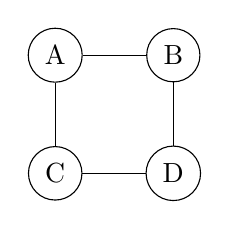
\begin{tikzpicture}[node distance=1.5cm, auto]
    \node[draw, circle] (A) {A};
    \node[draw, circle, right of=A] (B) {B};
    \node[draw, circle, below of=A] (C) {C};
    \node[draw, circle, right of=C] (D) {D};
    \draw (A) -- (B);
    \draw (A) -- (C);
    \draw (B) -- (D);
    \draw (C) -- (D);
\end{tikzpicture}
\end{center}

\textbf{BFS Pseudocode:}
\begin{lstlisting}
BFS(Graph, start):
    create a queue Q
    mark start as visited and enqueue start
    while Q is not empty:
        v = Q.dequeue()
        for all neighbors w of v:
            if w is not visited:
                mark w as visited
                enqueue w
\end{lstlisting}

\subsubsection{BFS C++ Implementation}
\begin{lstlisting}[caption={BFS in C++ using an Adjacency List}]
#include <iostream>
#include <vector>
#include <queue>
using namespace std;

void BFS(const vector<vector<int>>& adjList, int start) {
    int V = adjList.size();
    vector<bool> visited(V, false);
    queue<int> q;

    visited[start] = true;
    q.push(start);

    while (!q.empty()) {
        int v = q.front();
        q.pop();
        cout << v << " ";

        for (int neighbor : adjList[v]) {
            if (!visited[neighbor]) {
                visited[neighbor] = true;
                q.push(neighbor);
            }
        }
    }
}

int main() {
    vector<vector<int>> adjList = {
        {1, 2},    // Neighbors of 0
        {0, 2, 3}, // Neighbors of 1
        {0, 1, 3}, // Neighbors of 2
        {1, 2}     // Neighbors of 3
    };
    cout << "BFS Traversal starting from vertex 0:\n";
    BFS(adjList, 0);
    return 0;
}
\end{lstlisting}

\subsection{Depth-First Search (DFS)}
DFS is a traversal technique that explores as far as possible along each branch before backtracking. It is implemented using recursion or a stack.

\textbf{DFS Diagram:}
\begin{center}
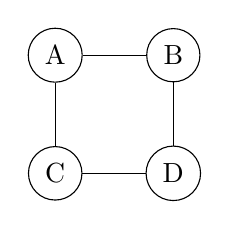
\begin{tikzpicture}[node distance=1.5cm, auto]
    \node[draw, circle] (A) {A};
    \node[draw, circle, right of=A] (B) {B};
    \node[draw, circle, below of=A] (C) {C};
    \node[draw, circle, right of=C] (D) {D};
    \draw (A) -- (B);
    \draw (A) -- (C);
    \draw (B) -- (D);
    \draw (C) -- (D);
\end{tikzpicture}
\end{center}

\textbf{DFS Pseudocode:}
\begin{lstlisting}
DFS(Graph, v):
    mark v as visited
    for all neighbors w of v:
        if w is not visited:
            DFS(Graph, w)
\end{lstlisting}

\subsubsection{DFS C++ Implementation}
\begin{lstlisting}[caption={DFS in C++ using an Adjacency List}]
#include <iostream>
#include <vector>
using namespace std;

void DFSUtil(const vector<vector<int>>& adjList, int v, vector<bool>& visited) {
    visited[v] = true;
    cout << v << " ";

    for (int neighbor : adjList[v]) {
        if (!visited[neighbor]) {
            DFSUtil(adjList, neighbor, visited);
        }
    }
}

void DFS(const vector<vector<int>>& adjList, int start) {
    int V = adjList.size();
    vector<bool> visited(V, false);
    DFSUtil(adjList, start, visited);
}

int main() {
    vector<vector<int>> adjList = {
        {1, 2},
        {0, 2, 3},
        {0, 1, 3},
        {1, 2}
    };
    cout << "DFS Traversal starting from vertex 0:\n";
    DFS(adjList, 0);
    return 0;
}
\end{lstlisting}

\section{Spanning Trees}

\subsection{Definition}
A \textbf{spanning tree} of a connected, undirected graph is a subgraph that is a tree and connects all the vertices together. A graph can have multiple spanning trees.

\subsection{Properties of Spanning Trees}
\begin{itemize}
    \item A spanning tree of a graph with $n$ vertices has exactly $n - 1$ edges.
    \item It is a minimal connected subgraph of the graph.
    \item There is no cycle in a spanning tree.
    \item Removing any edge from a spanning tree disconnects the graph.
    \item A connected graph with $n$ vertices and $n - 1$ edges is a tree.
\end{itemize}

\subsection{Minimum Spanning Tree (MST)}
A \textbf{minimum spanning tree} is a spanning tree whose sum of edge weights is the smallest among all possible spanning trees of the graph.

\textbf{Applications:}
\begin{itemize}
    \item Network design (e.g., electrical grid, computer networks)
    \item Approximation algorithms
    \item Clustering in machine learning
\end{itemize}

\textbf{Common Algorithms:}
\begin{itemize}
    \item \textbf{Kruskal's Algorithm}: Adds edges in increasing order of weight, skipping cycles.
    \item \textbf{Prim's Algorithm}: Grows the MST one vertex at a time from a starting node.
\end{itemize}

\subsection{Maximum Spanning Tree}
A \textbf{maximum spanning tree} is similar to an MST but maximizes the total edge weight. It is useful in certain optimization problems where higher weights are preferred (e.g., maximizing reliability or capacity).

\subsection{Comparison}
\begin{center}
\begin{tabular}{|l|l|l|}
\hline
\textbf{Aspect} & \textbf{MST} & \textbf{MaxST} \\
\hline
Objective & Minimize total weight & Maximize total weight \\
\hline
Used In & Cost-saving applications & Capacity or reliability maximization \\
\hline
Algorithm Change & Sort edges by increasing weight & Sort edges by decreasing weight \\
\hline
\end{tabular}
\end{center}
A \textbf{spanning tree} of a graph is a subgraph that includes all the vertices of the original graph, is connected, and has no cycles. In an undirected graph, any spanning tree will have exactly \( V - 1 \) edges.

\subsubsection{Example and Diagram of a Spanning Tree}
Given an undirected graph:
\begin{center}
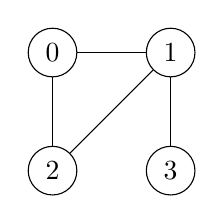
\begin{tikzpicture}[node distance=1.5cm, auto]
    \node[draw, circle] (0) {0};
    \node[draw, circle, right of=0] (1) {1};
    \node[draw, circle, below of=0] (2) {2};
    \node[draw, circle, right of=2] (3) {3};
    \draw (0) -- (1);
    \draw (0) -- (2);
    \draw (1) -- (2);
    \draw (1) -- (3);
\end{tikzpicture}
\end{center}

A possible spanning tree for the graph is:
\begin{center}
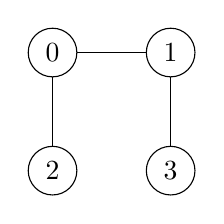
\begin{tikzpicture}[node distance=1.5cm, auto]
    \node[draw, circle] (0) {0};
    \node[draw, circle, right of=0] (1) {1};
    \node[draw, circle, below of=0] (2) {2};
    \node[draw, circle, right of=2] (3) {3};
    \draw (0) -- (1);
    \draw (0) -- (2);
    \draw (1) -- (3);
\end{tikzpicture}
\end{center}

\subsubsection{Spanning Tree via BFS (C++ Implementation)}
Below is an example of using BFS to generate a spanning tree from a connected undirected graph.
\begin{lstlisting}[caption={Spanning Tree using BFS in C++}]
#include <iostream>
#include <vector>
#include <queue>
using namespace std;

void spanningTreeBFS(const vector<vector<int>>& adjList, int start) {
    int V = adjList.size();
    vector<bool> visited(V, false);
    vector<int> parent(V, -1);
    queue<int> q;

    visited[start] = true;
    q.push(start);

    while (!q.empty()) {
        int u = q.front();
        q.pop();

        for (int v : adjList[u]) {
            if (!visited[v]) {
                visited[v] = true;
                parent[v] = u;
                q.push(v);
            }
        }
    }

    cout << "Spanning Tree (parent representation):\n";
    for (int i = 0; i < V; i++) {
        if (parent[i] != -1)
            cout << parent[i] << " - " << i << "\n";
    }
}

int main() {
    vector<vector<int>> adjList = {
        {1, 2},
        {0, 2, 3},
        {0, 1, 3},
        {1, 2}
    };
    spanningTreeBFS(adjList, 0);
    return 0;
}
\end{lstlisting}

\section{Diagrams for Graph Representations}

In this section, we provide visual diagrams for the two primary representations of graphs: the adjacency matrix and the adjacency list. We will consider a sample graph with vertices \(0,1,2,3\) and edges \(\{0,1\}\), \(\{0,2\}\), \(\{1,2\}\), and \(\{1,3\}\).

\subsection{Adjacency Matrix Diagram}
The adjacency matrix for the sample graph is a \(4 \times 4\) matrix where the rows and columns correspond to the vertices. A value of \(1\) indicates the presence of an edge between the corresponding vertices, and a value of \(0\) indicates no edge.

\begin{center}
\begin{tikzpicture}
  \matrix[matrix of nodes,
          nodes in empty cells,
          nodes={draw, minimum size=1cm, anchor=center},
          column sep=0pt,
          row sep=0pt
         ] {
         \ & 0 & 1 & 2 & 3 \\
         0 & 0 & 1 & 1 & 0 \\
         1 & 1 & 0 & 1 & 1 \\
         2 & 1 & 1 & 0 & 0 \\
         3 & 0 & 1 & 0 & 0 \\
  };
\end{tikzpicture}
\end{center}

\subsection{Adjacency List Diagram}
The adjacency list represents the graph by listing each vertex followed by the vertices adjacent to it. For our sample graph, the adjacency list is as follows:
\[
\begin{array}{l}
0: \quad 1 \rightarrow 2 \\
1: \quad 0 \rightarrow 2 \rightarrow 3 \\
2: \quad 0 \rightarrow 1 \\
3: \quad 1 \\
\end{array}
\]

The diagram below visually represents this structure:

\begin{center}
\begin{tikzpicture}[node distance=1cm, every node/.style={draw, rectangle, rounded corners, minimum height=0.8cm}]
    % List nodes for vertex labels
    \node (v0) {0:};
    \node[right=1cm of v0] (v0list) {1};
    \node[right=0.5cm of v0list] (v0list2) {$\rightarrow$ 2};

    \node (v1) [below=of v0] {1:};
    \node[right=1cm of v1] (v1list) {0};
    \node[right=0.5cm of v1list] (v1list2) {$\rightarrow$ 2};
    \node[right=0.5cm of v1list2] (v1list3) {$\rightarrow$ 3};

    \node (v2) [below=of v1] {2:};
    \node[right=1cm of v2] (v2list) {0};
    \node[right=0.5cm of v2list] (v2list2) {$\rightarrow$ 1};

    \node (v3) [below=of v2] {3:};
    \node[right=1cm of v3] (v3list) {1};
\end{tikzpicture}
\end{center}

These diagrams help in visualizing the structural differences between the two common graph representations. The matrix provides a compact, fixed-size representation (especially useful for dense graphs), while the list provides a more flexible and space-efficient representation (especially useful for sparse graphs).

\section{Conclusion}
This chapter has provided an in-depth exploration of graph data structures and algorithms. We began with the theoretical foundations, key terminology, and useful formulas.